\documentclass{article}
\usepackage{graphicx} % Required for inserting images
\usepackage{amssymb}
\usepackage{amsmath}
\usepackage{setspace}
\usepackage{booktabs}
\usepackage{ulem}
\usepackage{array}
\setlength{\tabcolsep}{10pt}
\renewcommand{\arraystretch}{1.2}
\usepackage[top=2cm,bottom=2cm,left=2.5cm,right=2.5cm,marginparwidth=1.5cm]{geometry}

% Roman Numbers, \rmnum{} & \Rmnum{}
\makeatletter
\newcommand{\rmnum}[1]{\romannumeral #1}
\newcommand{\Rmnum}[1]{\expandafter\@slowromancap\romannumeral #1@}

\title{CSCI-SHU 360 Homework2}
\author{Ninghao Lu nl2752}
\date{2024 Fall}

\begin{document}

\maketitle

\section*{Exercise 1 Linear Regression and Convexity}
\subsection*{Solution:}
\begin{align*}
    L(w) &=  \lVert y - X w\rVert^2_2 \\
         &= (y - X w)^T(y - X w) \\
         &= y^T y - y^T X w - (X w)^T y + w^T X^T X w \\
         &= y^T y - 2 w^T X^T y + w^T X^T X w
\end{align*}
Now compute the partial derivative of $L(w)$ with regard to $w$ using directional derivative.
Since L(w) is differentiable, the directional derivative in the direction of unit vector u is:
\begin{align*}
    D_u L(w) &= \lim_{h \to 0} \frac{L(w + hu) - L(w)}{h} \\
                  &= \lim_{h \to 0} \frac{y^T y - 2 (w+hu)^T X^T y + (w+hu)^T X^T X (w+hu) - y^T y + 2 w^T X^T y - w^T X^T X w}{h} \\
                  &= \lim_{h \to 0} \frac{- 2 (w+hu)^T X^T y + (w+hu)^T X^T X (w+hu) + 2 w^T X^T y - w^T X^T X w}{h} \\
                  &= \lim_{h \to 0} \frac{(- 2w^T - 2h^Tu^T + 2w^T) X^T y + (w+hu)^T X^T X (w+hu) - w^T X^T X w}{h} \\
                  &= \lim_{h \to 0} \frac{(- 2h^Tu^T) X^T y + w^T X^T X (w+hu) + (hu) w^T X^T X (w+hu) - w^T X^T X w}{h} \\
                  &= \lim_{h \to 0} \frac{(- 2h^Tu^T) X^T y + w^T X^T X w + w^T X^T X (hu) + (hu) w^T X^T X (w+hu) - w^T X^T X w}{h} \\
                  &= \lim_{h \to 0} \frac{(- 2h^Tu^T) X^T y + w^T X^T X (hu) + (hu) w^T X^T X (w+hu)}{h} \\
                  &= (- 2 u^T) X^T y + w^T X^T X u + u w^T X^T X w + \lim_{h \to 0} u w^T X^T X hu \\ 
                  &= \nabla_w L(w) \cdot u = (\nabla_w L(w))^T u
\end{align*}
Thus $\nabla L(w) = - 2 X^T y + 2 X^T X w$. To find the Hessian matrix $\nabla_w^2 L(w)$, we need to compute the partial derivative of $\nabla_w L(w)$ with regard to $w$.
\begin{align*}
    \nabla_w^2 L(w) &= \frac{\partial}{\partial w} \nabla_w L(w) \\
                    &= -2 (\frac{\partial}{\partial w} X^T y) + 2 \frac{\partial}{\partial w} X^T X w\\
                    &= 2 X^T X
\end{align*}
To prove the linear regression loss function is convex in the parameters $w$: $L(w) = \lVert y - X w\rVert^2_2 $, we need to show its Hessian matrix is PSD.
Since X is full rank, then $X^T X$ is always PSD. \\ 
As a result, we can conclude that the linear regression loss function is convex in the parameters $w$: $L(w) = \lVert y - X w\rVert^2_2 $.

\section*{Exercise 2}
\subsection*{2.1 Solution:}
$S_{2-1}(r) = 2 \pi r, \ V_{2-1}(r) = 2 \pi r = \pi r^2$ \\
$S_{3-1}(r) = 4 \pi r^2, \ V_{3-1}(r) = \frac{4}{3} \pi r^3$

\subsection*{2.2 Solution:}
Verification: 
\[\frac{d}{dr}V_2(r)=\frac{d}{dr}\pi r^2=2\pi r=S_{2-1}(r)\]
\[\frac{d}{dr}V_3(r)=\frac{d}{dr}\frac{4}{3}\pi r^3=4\pi r^2=S_{3-1}(r)\]
This equation shows that the surface area is the derivative of the volume.
As a result, the surface area can be understood as the rate of change of the volume with regard to the radius r. Intuitively, when you
change the radius r by a small amount $\Delta r$, the increased/decreased amount in volume can be evaluated approximately by multiplying the original surface area $S_{m-1} (r)$ and the thickness $\Delta r$.
\[V_m (r + \Delta r) - V_m(r) \approx S_{m-1} \Delta r  \quad \text{when} \quad r \to 0\]  
As a result, this equation makes sense.

\subsection*{2.3 Solution:}
Since $V_m(r)$ is only dependent on $r^m$, we have $V_m(r) = r^m V_m(1)$. From 2.2 we learn that
\begin{align*}
    S_{m-1}(r) &= \frac{\partial}{\partial r}(r^m V_m(1)) \\
               &= m r^{m-1} V_m(1) + r^m \frac{\partial}{\partial r} V_m(1) \\
               &= m r^{m-1} V_m(1)
\end{align*}
Moreover, when r = 1, $\bar{S}_{m-1} = S_{m-1}(r) = m V_m(1)$ So m = 1 As a result, we have 
\[S_{m-1}(r) = m r^{m-1} V_m(1) = r^{m-1} (m V_m(1)) = r^{m-1} \bar{S}_{m-1}\]

\subsection*{2.4 Solution:}
We integrate the probability density over all points on the surface of the sphere $S_{m-1}(r)$, so $||x||^2 = r^2$, 
\begin{align*}
    \rho_m(r) &= \int p(x) dx = \int \frac{1}{(2\pi\sigma^2)^{m/2}}\exp(-\frac{||x||^2}{2\sigma^2})dx \\
              &= \int \frac{1}{(2\pi\sigma^2)^{m/2}}\exp(-\frac{r^2}{2\sigma^2})dx \\
              &= \frac{1}{(2\pi\sigma^2)^{m/2}}\exp(-\frac{r^2}{2\sigma^2}) \int dx \\
              &= \frac{1}{(2\pi\sigma^2)^{m/2}}\exp(-\frac{r^2}{2\sigma^2}) S_{m-1}(r) \\ 
              &= \frac{1}{(2\pi\sigma^2)^{m/2}}\exp(-\frac{r^2}{2\sigma^2}) r^{m-1} \bar{S}_{m-1}
\end{align*}

\subsection*{2.5 Solution:}
\begin{align*}
    \frac{d}{dr}\rho_m(r)&=\frac{\bar{S}_{m-1}}{(2\pi\sigma^2)^{m/2}}\left(\frac{d}{dr}\exp(-\frac{r^2}{2\sigma^2})\cdot r^{m-1}\right)\\
    &=\frac{\bar{S}_{m-1}}{(2\pi\sigma^2)^{m/2}}\left(\exp(-\frac{r^2}{2\sigma^2})\cdot -\frac{2r}{2\sigma^2}\cdot r^{m-1}+\exp(-\frac{r^2}{2\sigma^2})\cdot(m-1)\cdot r^{m-2}\right)\\
    &=\frac{\bar{S}_{m-1}}{(2\pi\sigma^2)^{m/2}}\cdot \exp(-\frac{r^2}{2\sigma^2})\cdot r^{m-2}\cdot\left(-\frac{r^2}{\sigma^2} + m - 1\right)
\end{align*}
Let $\frac{d}{dr}\rho_m(r) = 0$, we have $r = \sqrt{m-1} \sigma = \hat{r}$. When $r < \hat{r}$, $\frac{d}{dr}\rho_m(r) > 0$ so $\rho_m(r) \nearrow$ as r $\nearrow$ and when $r > \hat{r}$, $\frac{d}{dr}\rho_m(r) < 0$ so $\rho_m(r) \searrow$ as r $\searrow$
since $\frac{\bar{S}_{m-1}}{(2\pi\sigma^2)^{m/2}}\cdot \exp(-\frac{r^2}{2\sigma^2})\cdot r^{m-2} \geq 0$. Moreover, for large m, $\sqrt{m-1} \to \sqrt{m}$. As a result, $\frac{d}{dr}\rho_m(r)$ has a single maximum at $\hat{r}$ such that $\hat{r} \approx \sqrt{m} \sigma$.

\subsection*{2.6 Solution:}
\[\rho_m(\hat{r}) = \frac{1}{(2\pi\sigma^2)^{m/2}}\exp(-\frac{\hat{r}^2}{2\sigma^2}) \hat{r}^{m-1} \bar{S}_{m-1}\]
\[\rho_m(\hat{r} + \epsilon) = \frac{1}{(2\pi\sigma^2)^{m/2}}\exp(-\frac{(\hat{r} + \epsilon)^2}{2\sigma^2}) (\hat{r} + \epsilon)^{m-1} \bar{S}_{m-1}\]
As a result, 
\begin{align*}
    \frac{\rho_m(\hat{r} + \epsilon)}{\rho_m(\hat{r})} &= \frac{\frac{1}{(2\pi\sigma^2)^{m/2}}\exp(-\frac{(\hat{r} + \epsilon)^2}{2\sigma^2}) (\hat{r} + \epsilon)^{m-1}}{\frac{1}{(2\pi\sigma^2)^{m/2}}\exp(-\frac{\hat{r}^2}{2\sigma^2}) \hat{r}^{m-1}} \\
                                                       &= \exp(-\frac{2 \hat{r} \epsilon + \epsilon^2}{2 \sigma^2}) (1 + \frac{\epsilon}{\hat{r}})^{m-1}                                       
\end{align*}
By Taylor's Expansion, $ln(1+x) = \sum_{n=1}^{\infty} (-1)^n \frac{x^n}{n} = x - \frac{x^2}{2} + \dots$. We notice that similar pattern appears in $(1 + \frac{\epsilon}{\hat{r}})^{m-1}$. Since $\epsilon << \hat{r}, \frac{\epsilon}{\hat{r}} \to 0$ and from 2.5 we have that m - 1 = $(\frac{\hat{r}}{\sigma})^2$
\begin{align*}
    (1 + \frac{\epsilon}{\hat{r}})^{m-1}  &= e^{ln (1 + \frac{\epsilon}{\hat{r}})^{m-1}} \\
                                          &= e^{(m - 1) ln (1 + \frac{\epsilon}{\hat{r}})} \\
                                          &\approx e^{(m - 1) (\frac{\epsilon}{\hat{r}} - \frac{(\frac{\epsilon}{\hat{r}})^2}{2})} \\
                                          &= e^{(\frac{\hat{r}}{\sigma})^2 (\frac{\epsilon}{\hat{r}} - \frac{(\frac{\epsilon}{\hat{r}})^2}{2})} \\
                                          &= exp(\frac{\hat{r} \epsilon}{\sigma^2} - \frac{\epsilon^2}{2 \sigma^2})
\end{align*}  
Therefore,  
\begin{align*}
    \frac{\rho_m(\hat{r} + \epsilon)}{\rho_m(\hat{r})} &\approx \exp(-\frac{2 \hat{r} \epsilon + \epsilon^2}{2 \sigma^2}) \cdot exp(\frac{\hat{r} \epsilon}{\sigma^2} - \frac{\epsilon^2}{2 \sigma^2}) \\
                                                       &= \exp(-\frac{\epsilon^2}{\sigma^2})
\end{align*}
Thus, $\rho_m(\hat{r} + \epsilon) \approx \rho_m(\hat{r}) \exp(-\frac{\epsilon^2}{\sigma^2})$.

\subsection*{2.7 Solution:}
From problem 2.5 we learn that in a high dimensional Gaussian distribution, $\rho_m(r)$ gets its maximum when r = $\hat{r} \approx \sqrt{m} \sigma$. Since it is in high dimensional space, m is quite large. Therefore,  most of the points reside far away from the $\sigma$ neighbourhood at the radius of r = $\hat{r} \approx \sqrt{m} \sigma$.
For a low dimensional Gaussian distribution, most points reside with the $\sigma$ neighbourhood at the radius of r = $\sqrt{m-1} \sigma$.

\subsection*{2.8 Solution:}
Calculate and compare the probability density at the origin and at one point on sphere $S_{m-1}(\hat{r})$:\\
At the origin, the probability density is
\[p(0) = \frac{1}{(2 \pi \sigma^2)^(m/2)}\]
At one point $x_0$ on sphere $S_{m-1} (\hat{r})$, where the radius is $\hat{r} \approx \sqrt{m}\sigma$ the probability density is
\[p(x_0) = \frac{1}{(2 \pi \sigma^2)^(m/2)} \exp(-m^2 / 2)\]
We can see that $p(0) > p(x_0)$, that is, the probability density at one point $x_0$ on sphere $S_{m-1} (\hat{r})$ is smaller than that at the origin.
\begin{figure}[h]
    \centering
    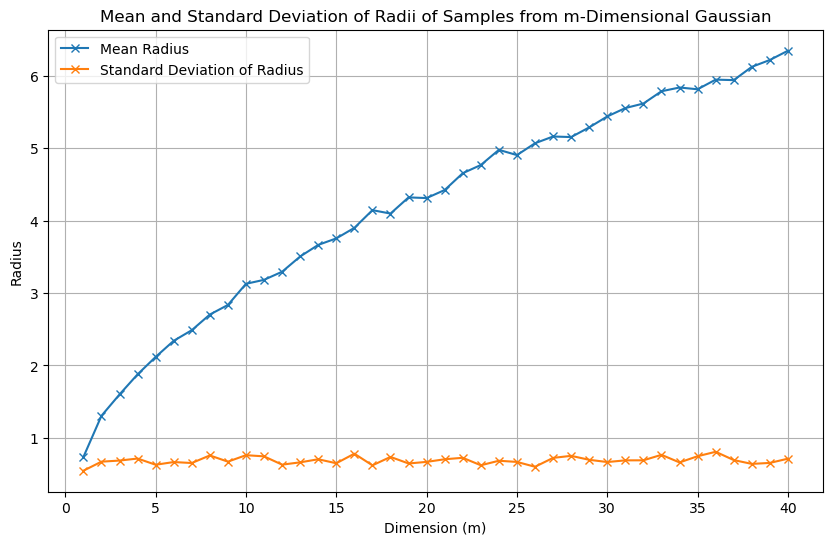
\includegraphics[width=0.5\linewidth]{/Users/luninghao/Documents/Study/CS & DS/CSCI-SHU 360 Machine Learning/Homework/HW2/2.8.png}
    % \caption{}
    % \label{fig: 6.1} 
\end{figure}\\
From the figure above we can see that my plot is consistent with the above since approximately the radius follows the formula $\hat{r} \approx \sqrt{m} \sigma$ when the dimensionality is high. That means, in higher dimensionality, most points would reside in some radius that is far away from origin.
Although the probability density at the origin remains high ($p(0) > p(x_0)$), the overall probability mass shifts away from the origin to the radius $\hat{r}$.
Moreover, since the standard deviation doesn't change much, we can derive that in high dimensions most points would gather around at this spherical shell far from the origin.

\newpage
\section*{Exercise 3 Ridge Regression}
\subsection*{3.1 Solution:}
\begin{figure}[h]
    \centering
    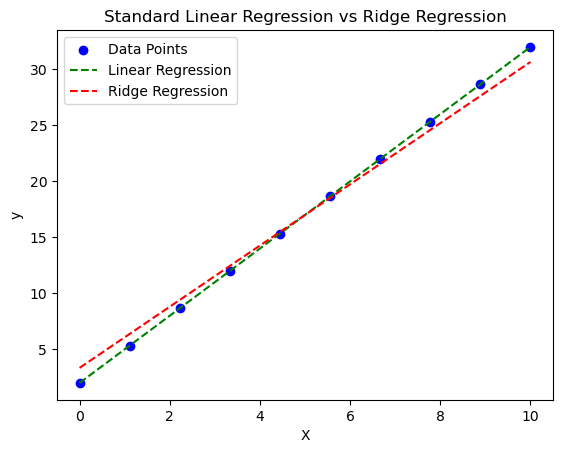
\includegraphics[width=0.5\linewidth]{/Users/luninghao/Documents/Study/CS & DS/CSCI-SHU 360 Machine Learning/Homework/HW2/3.1.png}
    % \caption{}
    % \label{fig: 6.1} 
\end{figure}
Take the setting where the relationship bewteen X and y are perfectly linear, (In my example y = 3X + 2). 
Standard linear regression is preferred because it provides exact solution by minimizing the loss function and there is no need for regularization since the standard linear model can fit the data without the risk of overfitting.



\subsection*{3.2 Solution:}
\begin{figure}[h]
    \centering
    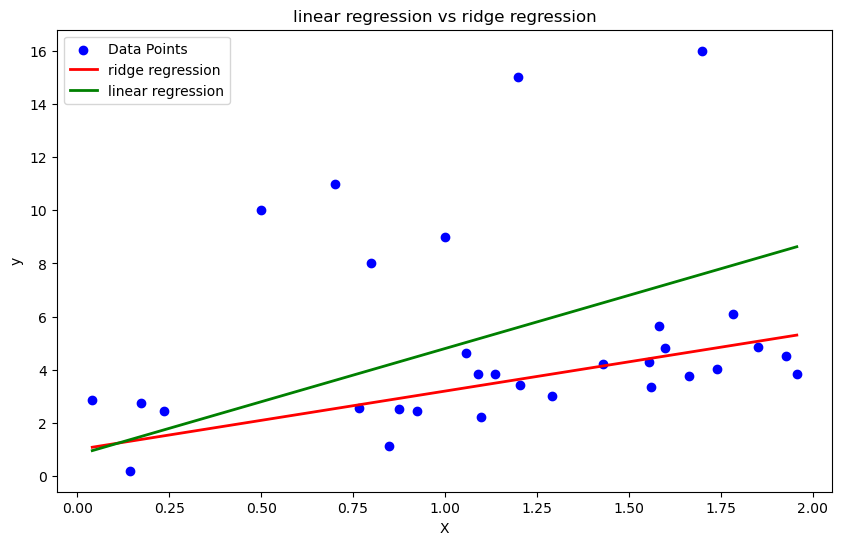
\includegraphics[width=0.5\linewidth]{/Users/luninghao/Documents/Study/CS & DS/CSCI-SHU 360 Machine Learning/Homework/HW2/3.2.png}
    % \caption{}
    % \label{fig: 6.1} 
\end{figure}
When there are more outliers in the setting, ridge regression is more preferred than linear regression because it is more robust to outliers as it can adjust its coefficients through the regularization term.
However, outliers can significantly impact the coefficients of linear regression, making the model doesn't generalize well to new data.




\subsection*{3.3 Solution:}
Let
\begin{align*}
    L(w) &= ||Xw - y||_2^2 + \frac{\eta}{2} ||w||_2^2 \\
         &= (Xw - y)^T (Xw - y) + \frac{\eta}{2} ||w||_2^2 \\
         &= w^T X^T X w - y^T Xw - X w y + y^T y
\end{align*}
To find its closed-form solution, from 1 we know that 
\begin{align*}
    \nabla_w L(w) &= - 2 X^T y + 2 X^T X w + \nabla (\frac{\eta}{2} ||w||_2^2) \\
                &= - 2 X^T y + 2 X^T X w + \eta I w
\end{align*}
Moreover, from Problem 1 we learn that, $\nabla_w^2 L(w) = 2 X^T X + \eta I$. Since $\eta > 0$, $\nabla_w^2 L(w) > 0$, $\nabla_w L(w)$ is a convex function.
As a result, we set $\nabla_w L(w) = 0$, we have
\begin{align*}
        \nabla_w L(w) = - 2 X^T y + 2 X^T X w + \eta I w &= 0 \\
             2 X^T X w + \eta I w &= 2 X^T y \\
             (2 X^T X + \eta I) w = 2 X^T y
\end{align*}
Therefore, the closed-form solution for ridge regression is w = $(2 X^T X + \eta I)^{-1} 2 X^T y$

\subsection*{3.4 Solution:}
\subsubsection*{For case (1) where the columns (or features) of X are more than the rows (or samples)}
\subsubsection*{(a)}
Since the columns of X are more than the rows of X, X is not full rank. X is not invertible. Thus, the matrix $X^T X$ is not invertible. We cannot directly compute the closed-form solution $w = (X^T X)^{-1} X^T y$.
\subsubsection*{(b)}
From (a) we learn that $X^T X$ is not invertible. From the perspective of eigenvalue, this means $X^T X$ has its eigenvalue(s) be 0. However, after introducing the regularization term, making it be $2 X^T X + \eta I$ with $\eta > 0$. 
We can see that the eigenvalues will be positive since the original positions on the main diagonal where eigenvalues being 0 are added the positive number $\eta$, thus making the eigenvalues no longer being zero. As a result, $2 X^T X + \eta I$ becomes invertible. This makes us always able to compute the closed-form of ridge regression.
\subsubsection*{For case (2) where the columns (or features) of X are highly correlated (an extreme case is where many features are identical to each other)}
\subsubsection*{(a)}
Since the columns of X are highly correlated, the columns of X are not linearly independent. So X is also not full rank. X is not invertible. Thus, the matrix $X^T X$ is not invertible. We cannot directly compute the closed-form solution $w = (X^T X)^{-1} X^T y$.
\subsubsection*{(b)}
The same reason as case(1)(b).
In conclusion, other benefit of ridge regression is that it can always give us solutions when we are dealing with problems where features are highly correlated or the number of features are greater than the number of examples.

\newpage
\section*{Exercise 4 Locality Sensitive Hashing}
\subsection*{4.1 Solution:}
Intuitively, r represents the distance within which we expect to find a point that is close to the query point. c is a scaling factor that determines how far the magic oracle is allowed to extend its returned result.\\
\textbf{Step 1: Choose an initial guess for \( r \) and c}

We can start by setting a relatively large value of \( r \) and for the exact nearest neighbor search, we want to minimize the approximation error, so we should set \( c \) as close to 1 as possible (i.e., \( c = 1 + \epsilon \) for a small \( \epsilon > 0 \)).

\textbf{Step 2: Adjust \( r \) using binary search}

We now perform a binary search on the value of \( r \) in the range of [0, m] to shrink \( r \) progressively, while ensuring that the oracle still returns a point \( x' \in X \) with \( d(x', q) \leq cr \).

Start with an upper bound \( r_{\text{max}} = m \) and a lower bound \( r_{\text{min}} = 0 \).
Set \( r = \frac{r_{\text{max}} + r_{\text{min}}}{2} \) and call the oracle with this value of \( r \).
If the oracle returns a point \( x' \), update \( r_{\text{max}} = r \). If the oracle returns nothing, update \( r_{\text{min}} = r \), as no points exist within \( cr \) distance. Continue this binary search until \( r_{\text{max}} - r_{\text{min}} \) is sufficiently small and this is when the returned point is the nearest neighbor.

\subsection*{4.2 Solution:}
We know that the hash function h will map $x_i, x_j$ to the same value if $x_i$'s and $x_j$'s elements of selected indexes are the same.
For the lower bound, if \( d(x_i, x_j) \leq r \), this means that there are at most $r$ positions where \(x_i\) and \(x_j\) differ.
Thus, the probability that the hash function h selects a coordinate where \( x_i \) and \( x_j \) are the same is given by
\[ p_1 = \frac{m - r}{m} \]

For the upper bound, if \( d(x_i, x_j) \geq c r \), this means that there are at least $cr$ positions where \(x_i\) and \(x_j\) differ.
Thus, the probability that the hash function h selects a coordinate where \( x_i \) and \( x_j \) are the same is given by
\[ p_2 = \frac{m - c r}{m} \]

\subsection*{4.3 Solution:}
We know that the new hash function g (including k hash fucntions) will map $x_i, x_j$ to the same value if the corresponding hash functions of $x_i$ and $x_j$ are the same. \\
For the lower bound, if \( d(x_i, x_j) \leq r \), this means that there are at most $r$ positions where \(x_i\) and \(x_j\) differ. For each hash function, we learn from 4.2 the lower bound of a hash function h selects a coordinate where \( x_i \) and \( x_j \) are the same is given by $p_1$. Therefore, 
\begin{align*}
    Pr(g(x_i) = g(x_j)) &= Pr((h_1(x_i) = h_1(x_j)) \land (h_2(x_i) = h_2(x_j)) \land ... \land (h_k(x_i) = h_k(x_j)))\\
                        &= Pr((x_i[a_1] = x_j[a_1]) \land (x_i[a_2] = x_j[a_2]) \land ... \land (x_i[a_k] = x_j[a_k]))\\
                        &= Pr((x_i[a_1] = x_j[a_1]))Pr((x_i[a_2] = x_j[a_2]))...Pr((x_i[a_k] = x_j[a_k]))\\
                        &\geq p_1^k
\end{align*} So the lower bound for the probability that $g(x_i) = g(x_j)$ if \( d(x_i, x_j) \leq r \) is $p_1^k$.\\
For the upper bound, if \( d(x_i, x_j) \geq c r \), this means that there are at least $c r$ positions where \(x_i\) and \(x_j\) differ. For each hash function, we learn from 4.2 the upper bound of a hash function h selects a coordinate where \( x_i \) and \( x_j \) are the same is given by $p_2$. Therefore, 
\begin{align*}
    Pr(g(x_i) = g(x_j)) &= Pr((h_1(x_i) = h_1(x_j)) \land (h_2(x_i) = h_2(x_j)) \land ... \land (h_k(x_i) = h_k(x_j)))\\
                        &= Pr((x_i[a_1] = x_j[a_1]) \land (x_i[a_2] = x_j[a_2]) \land ... \land (x_i[a_k] = x_j[a_k]))\\
                        &= Pr((x_i[a_1] = x_j[a_1]))Pr((x_i[a_2] = x_j[a_2]))...Pr((x_i[a_k] = x_j[a_k]))\\
                        &\leq p_2^k
\end{align*} So the upper bound for the probability that $g(x_i) = g(x_j)$ if \( d(x_i, x_j) \geq c r \) is $p_2^k$.

\subsection*{4.4 Solution:}
The lower bound for the probability that $\exists$ b $\in \{0, 1, \dots, l-1\} \text{ such that } g_b(x_i) = g_b(x_j) \text{ if } d(x_i, x_j) \leq r \text{ can be transformed as:}$
\begin{align*}
    Pr(\exists b, g_b(x_i) = g_b(x_j)) &= 1 - Pr(g_0(x_i) \neq g_0(x_j))Pr(g_1(x_i) \neq g_1(x_j)) \dots Pr(g_{l-1}(x_i) \neq g_{l-1}(x_j))\\
                                       &= 1 - (Pr(g_b(x_i) \neq g_b(x_j)))^l \\
                                       &= 1 - (1 - Pr(g_b(x_i) = g_b(x_j)))^l\\
                                       &\geq 1 - (1 - p_1^k)^l
\end{align*}
So a lower bound is $1 - (1 - p_1^k)^l$.\\
The upper bound for the probability that $\exists$ b $\in \{0, 1, \dots, l-1\} \text{ such that } g_b(x_i) = g_b(x_j) \text{ if } d(x_i, x_j) \geq cr \text{ can be transformed as:}$
\begin{align*}
    Pr(\exists b, g_b(x_i) = g_b(x_j)) &= 1 - Pr(g_0(x_i) \neq g_0(x_j))Pr(g_1(x_i) \neq g_1(x_j)) \dots Pr(g_{l-1}(x_i) \neq g_{l-1}(x_j))\\
                                       &= 1 - (Pr(g_b(x_i) \neq g_b(x_j)))^l\\
                                       &= 1 - (1 - Pr(g_b(x_i) = g_b(x_j)))^l\\
                                       &\leq 1 - (1 - p_2^k)^l
\end{align*} So a upper bound is $1  - (1 - p_2^k)^l$.

\subsection*{4.5 Solution:}
\subsubsection*{(a)}
From 4.4, since $d(x', q) \leq r$, and from given conditions in 4.5 we have that 
\[Pr(\exists b, g_b(x_i) = g_b(x_j)) \geq 1 - (1 - p_1^k)^l = 1 - (1 - p_1^{\frac{ln(n)}{ln(1/p_2)}})^{n^{\frac{ln(p_1)}{ln(p_2)}}}\]
Moreover, 
\[p_1^{\frac{ln(n)}{ln(1/p_2)}} = e^{ln(p_1^{\frac{ln(n)}{ln(1/p_2)}})} = e^{-\frac{ln(n) ln(p_1)}{ln(p_2)}} = (n^{\frac{ln(p_1)}{ln(p_2)}})^{-1} = k^{-1}\]
Therefore, $1 - (1 - p_1^k)^l = 1 - (1 - p_1^{\frac{ln(n)}{ln(1/p_2)}})^{n^{\frac{ln(p_1)}{ln(p_2)}}}$ becomes $(1 - \frac{1}{k})^k$. Since $(1 - 1/k)^k < e^{-1}$,
We get the conclusion that 
\[Pr(\exists b, g_b(x_i) = g_b(x_j)) \geq 1 - (1 - 1/k)^k > 1 - e^{-1}\] which means the first event happens with the probability at least $1 - e^{-1}$.


\subsubsection*{(b)}
Let X denote the number of x $\in$ X such that $d(x,q) \geq cr$ and $g_b(x) = g_b(q)$. Using Markov inequality, we have
\[P(X \geq 4l) \leq \frac{E(X)}{4l}\]
Moreover, since $E[X] = \sum_{x} x P(X = x)$, and from 4.4 we learn that 
\begin{align*}
    E(X) &= n Pr(\exists b, g_b(x_i) = g_b(x_j)) \\
         &\leq n(1 - (1 - p_2^k)^l) = n (1 - ( 1 - p_2^{\frac{ln(n)}{ln(1/p_2)}})^l) = n(1 - (1 - e^{\frac{ln(n) ln(p_2)}{-ln(p_2)}} )^l)\\
         &= n(1 - (1 - 1/n)^l) \approx n(1 - 1 + l / n) = l
\end{align*} 
Thus, $P(X \geq 4l) \leq \frac{E(X)}{4l} = l / 4l = 1 / 4$ \\
Therefore $P(X \leq 4l) = 3 / 4$.

Since the two events are independent as it is impossible for one data point to satisfy $d(x,q) \geq cr$ and $d(x,q) \leq r$ simultaneously, 
the lower bound of the probability that both events happen is $(3/4 (1 - e^{-1}))$.





\subsection*{4.6 Solution:}
Since the two events in 4.5 happened with certainty, we only need to check 4n + 1 points to ensure that we are returned with a point that has distance at most $cr$ to the query point becasue there are at most 4l points in X such that  $d(x,q) \geq cr$ and $g_b(x) = g_b(q)$.\\
We are guarenteed that there is a point with distance at most $cr$ becasue since event(a) from 4.4 happens with certainty, we will be returned with some $x' \in X$, $d(x',q) \leq r$, $\exists$ b $\in \{0, 1, \dots, l-1\} \text{ such that } g_b(x_i) = g_b(x_j). \text{ Since } d(x', q) \leq r$, it also satisfies $d(x', q) \leq cr$. This is why we are guarenteed to be returned such a point.




\newpage
\section*{Exercise 5 Linear Regression}
\subsection*{5.1 Solution:}
The top 3 features are \textbf{LSTAT}, \textbf{RM} and \textbf{PTRATIO} because they look most linearly related to price in their scatter plots.

\subsection*{5.2 Solution:}
According to the correlation matrix and heatmap, we can see that the top-3 features that are mostly (linearly) related to the house price (“MEDV”) are
\textbf{LSTAT} ($\rho \approx -0.737663$), \textbf{RM} ($\rho \approx 0.695360$) and \textbf{PTRATIO} ($\rho \approx -0.507787$).
It is quite fortunate that the result is the same as that in 5.1 because from the matrix we can see that the correlation coefficient between feature $\textbf{INDUS}$ and price is quite close to \textbf{PTRATIO}'s, which may mislead our judgment in 5.1.

\subsection*{5.3 Solution:}
After implementing the linear regression and ridge regression, we obtain coefficients $w$ in the following table.
\begin{table}[h]
    \centering
    \caption{Coefficient $w$ for Linear and Ridge Regression}
    \label{tab:coefficients}
    \begin{tabular}{lcccc}
    \toprule
    Features & \multicolumn{1}{l}{Linear Regression} & \multicolumn{3}{c}{Ridge Regression} \\
    \cmidrule(r){2-2} \cmidrule(r){3-5}
     & $\eta = 0$ & $\eta = 5.0$ & $\eta = 15.0$ & $\eta = 90.0$ \\
    \midrule
    CRIM    & -0.099324 & -0.100368 & -0.101157 & -0.100959 \\
    ZN      & 0.052251  & 0.053839  & 0.056906  & 0.073367  \\
    INDUS   & 0.004516  & 0.011329  & 0.016161  & 0.021451  \\
    CHAS    & 2.957261  & 2.462736  & 1.854801  & 0.720841  \\
    NOX     & 1.127938  & 0.513974  & 0.380824  & 0.231915  \\
    RM      & 5.854198  & 5.778194  & 5.574767  & 4.337233  \\
    AGE     & -0.014957 & -0.011505 & -0.006243 & 0.019888  \\
    DIS     & -0.920844 & -0.906153 & -0.869514 & -0.653085 \\
    RAD     & 0.159519  & 0.162332  & 0.164159  & 0.155832  \\
    TAX     & -0.008934 & -0.008962 & -0.008988 & -0.008030 \\
    PTRATIO & -0.435674 & -0.416153 & -0.375560 & -0.125780 \\
    B       & 0.014905  & 0.015341  & 0.015989  & 0.019100  \\
    LSTAT   & -0.474751 & -0.480413 & -0.495622 & -0.577238 \\
    \bottomrule
    \end{tabular}
    \end{table}\\
From the table we can see that after inrtoducing ridge regression, as $\eta$ gets larger, most features' absolute value of coefficient $w$ gets smaller, which coincides with the effect of ridge regression.

\subsection*{5.4 Solution:}
After implementation, we obtain results as follows:
\begin{table}[h]
    \centering
    \caption{RMSE of Linear and Ridge Regression at Various Levels of Regularization}
    \label{tab:my_label}
    \begin{tabular}{@{}lcccc@{}}
    \toprule
    Dataset & Linear Regression & \multicolumn{3}{c}{Ridge Regression} \\
    \cmidrule(l){2-2} \cmidrule(l){3-5}
    & $\eta = 0$ & $\eta = 5.0$ & $\eta = 15.0$ & $\eta = 90.0$ \\
    \midrule
    Train Set & 4.8206 & 4.8235 & 4.8379 & 5.0411 \\
    Test Set  & 5.2092 & 5.1941 & 5.1878 & 5.3017 \\
    \bottomrule
    \end{tabular}
    \end{table}\\
Comparing the training RMSE of linear regression and ridge regression, we can see that as $\eta$ gets larger, the RMSE gets larger as well. 
However, as $\eta$ gets larger, the test RMSE gets smaller then it becomes larger. \\
Possible explanation for this is that:\\
For training RMSE, larger $\eta$ lead to stronger penalization of the coefficients, making the model less able to fit the training data closely, which results in higher errors.
For test RMSE, initially when $\eta$ increases, it can help the model be more flexible and reduce overfitting thus makes the error smaller. However, $\eta$'s excessive growth will lead to the model's underfitting of the data, which is represented by larger test RMSE.

\subsection*{5.5 Solution:}
Using the top 3 features to train a linear regression model and a ridge regression model, I obtained the following results:

\begin{table}[h]
    \centering
    \caption{RMSE of Linear and Ridge Regression using Top 3 Features}
    \label{tab:rmse_top3}
    \begin{tabular}{lcc}
    \toprule
    \textbf{Dataset}  & \textbf{Linear Regression} & \textbf{Ridge Regression ($\eta = 15.0$)} \\
    \midrule
    \textbf{Train Set} & 5.2734 & 5.2798 \\
    \textbf{Test Set}  & 5.4947 & 5.4717 \\
    \bottomrule
    \end{tabular}
\end{table}

By comparing the RMSE of using all 13 features, we can see that the RMSE values are quite similar. This indicates that using only the top 3 features for prediction still results in good model performance. The top 3 features capture most of the significant information required to predict house prices, and the remaining features may have limited impact. 

Moreover, reducing the dimensionality of this problem leads to faster computation and lower complexity while maintaining similar performance.


\end{document}